% !TeX spellcheck = fr_FR

\chapter{Chapitre 4 : Résultats}
Dans ce chapitre, nous allons voir les résultats obtenus par les
différentes parties de l'application. On va aussi comparer les différentes
métriques collectés des binaires.

Les tests suivants ont été réaliser principalement sur la configuration d'ordinateur
se trouvant dans la figure \ref{fig:computer_configuration} en annexe 4.

\section{Triangulation}

La triangulation de Delaunay provient en grande partie du projet de semestre.
Seule la partie fusion de maillage a été implémenté dans ce travail.

Pour la triangulation, on utilise deux fichiers:
\begin{itemize}
	\item Le fichier 2501500\_1112000.las du jeu de données des \gls{sitg} contenant 9'000'987 points
	\item Un fichier contenant que les 100'000 premiers points du fichier précédent.
\end{itemize}

\subsection{Algorithme de Bowyer-Watson}

\begin{table}[htbp!]
	\begin{tabular}{l|c|c|c|c|}
		\cline{2-5}
		\multicolumn{1}{c|}{}                              & Nb Points                    & \begin{tabular}[c]{@{}c@{}}Temps moyen\\ {[}s{]}\end{tabular} & Nb Trig                     & \begin{tabular}[c]{@{}c@{}}Taille de sortie\\ {[}Mb{]}\end{tabular} \\ \hline
		\multicolumn{1}{|l|}{2501500\_1112000\_sample.las} & \multicolumn{1}{l|}{100'000} & \multicolumn{1}{l|}{6,646082286}                              & \multicolumn{1}{l|}{199928} & 9.6 Mb                                                              \\ \hline
		\multicolumn{1}{|l|}{2501500\_1112000.las}         & 9'000'987                    & N/A                                                           & N/A                         & N/A                                                                 \\ \hline
	\end{tabular}
	\caption{Résultats de la triangulation avec l'algorithme Bowyer-Watson}
	\label{tab:triangulation_results}
\end{table}

Dans le tableau \ref{tab:triangulation_results}, on peut observer que sur un
fichier de plusieurs millions de points aucune valeur n'est présente. L'implémentation actuel n'arrivant pas à
exécuté en un temps raisonnable, les valeurs ici manque.

\subsection{Algorithme Delaunator}

Cette partie utilise une implémentation de la triangulation de delaunay
existante. Il s'agit de l'algorithme delaunator implémentant des idées de S-hull
et de sweepline triangulation.

Les résultats suivants montre l'efficacité de cet implémentation par rapport à
l'implémentation de Bowyer-Watson.

\begin{table}[htbp!]
	\begin{tabular}{l|c|c|c|c|}
		\cline{2-5}
		\multicolumn{1}{c|}{}                              & Nb Points                    & \begin{tabular}[c]{@{}c@{}}Temps moyen\\ {[}s{]}\end{tabular} & Nb Trig                      & \begin{tabular}[c]{@{}c@{}}Taille de sortie\\ {[}Mb{]}\end{tabular} \\ \hline
		\multicolumn{1}{|l|}{2501500\_1112000\_sample.las} & \multicolumn{1}{l|}{100'000} & \multicolumn{1}{l|}{0,0512579617}                             & \multicolumn{1}{l|}{199'928} & 9.6                                                                 \\ \hline
		\multicolumn{1}{|l|}{2501500\_1112000.las}         & 9'000'987                    & 9,547529753                                                   & 18'001'310                   & 859                                                                 \\ \hline
	\end{tabular}
	\caption{Résultats de la triangulation avec l'algorithme delaunator}
	\label{tab:triangulation_delaunator_result}
\end{table}

\subsection{Fusion de triangulation}

Les résultats de la fusion ne sont pas disponible car le binaire actuel ne
soummet pas de fichier de sortie.

On peut observer le flamegraph de la figure \ref{fig:flamegraph_mesh_merge}
du binaire ou le programme reste bloqué dans la méthode \textit{get\_side\_candidate}
avant que ce dernier soit intérompu.

\begin{figure}[htbp!]
    \centering
    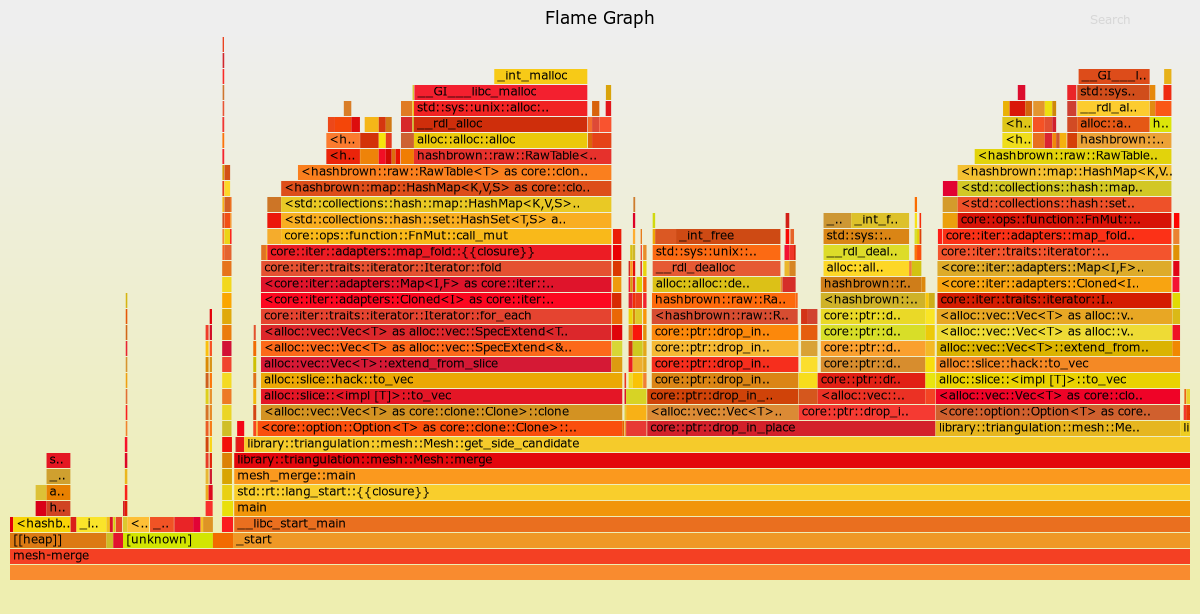
\includegraphics[width=0.8\linewidth]{figures/merge-debug-flamegraph.png}
    \caption{Flamegraph du binaire mesh-merge. Source : réalisé par Jérôme Chételat}
    \label{fig:flamegraph_mesh_merge}
\end{figure}


Cependant les tests unitaires valide l'algorithme pour un jeu de données simple.

\textbf{Améliorations possibles}

L'implémentation actuelle gère uniquement les maillages linéairement séparable.
L'idée serait de pouvoir aussi gérer le cas ou les maillages peuvent se
supperposé.

On a aussi le problème que l'algorithme ne s'applique que dans une direction
pour créer des arrêtes. Le principe serait d'implémenter un choix de direction
pour appliqué la fusion.

\section{Nettoyage}

\subsection{Point moyen}
\subsection{Point pondéré}

\subsection{Lissage de maillage}
\subsection{Décimation de maillage}

\section{Stack Web}
\subsection{Serveur Web}

Le serveur actuel permet les téléchargements de fichiers \gls{stl} présent dans
un dossier spécifique. 

\subsection{Client Web}
Les tests suivants ont été effectué sur les navigateur Firefox version 81 et
Chromium version.
Le client web permet actuellement de faire un rendu d'un maillage dans un
navigateur web. Un fichier \gls{stl} est téléchargé à l'aide de l'api
\textit{fetch} du navigateur au chargement de la page web.

\textbf{Amélioration possible} \\
Le chargement des vertex du maillage se faisant dans un seul file d'exécution,
la page lors du chargement reste figée et peut ne plus répondre (dépend de la
puissance de l'hôte) .
Il serait possible dans un futur proche de faire ces opérations dans des WebWorkers. Au
moment de l'écriture de ce mémoire, les possibilités d'utiliser des WebWorkers
en Rust est encore expérimental.
